\part{基本初等函数}
欢迎来到这本讲义的第三部分。在前两部分中我们解决了高中数学中最基础的部分，而从这里开始
要上难度了。首先 
\chapter{函数与映射初步}
\section{映射*}
\subsection{定义，分类，例子}
\subsection{映射的复合}

\clearpage
\section{函数的基本概念}
\subsection{函数的基本概念及其三要素}

\begin{definition}[函数，定义域，值域]
    \ 

    函数$f(\cdot)$是指从非空数集$A$到非空数集$B$的映射$f$.
    其中映射的定义域$A$称为函数$f(\cdot)$的定义域，映射的值域称作$f(\cdot)$的值域.
\end{definition}
\begin{zhu}
    在映射中，我们可能会经常研究一些不满的映射，这意味着陪域和值域不等。
    而在函数中，我们会默认把陪域缩小到值域的大小。当然这种问题是很trivial的，不必纠结。
\end{zhu}
我们在初中阶段学习了一次函数，二次函数和反比例函数。现在我们用定义域和值域的语言来叙述一下。
\begin{example}
    \ 

    $(1)$一次函数

    一次函数$f(x)=kx+b(k\neq0)$的定义域和值域都是$\mathbb{R}$，也常写作$(-\infty,+\infty)$.
    
    $(2)$二次函数

    $(3)$反比例函数
\end{example}
原像构成的集合，更功利化的一句话总结是：“定义域是x的取值范围”。这本身是句废话，但是在复合函数的地方我们会看到这句话的用处。

一些常见的限制：根号，分式，零次幂，对数
\begin{definition}[复合函数]
    
\end{definition}
\begin{example}
    \ 

    $f(x+1)$的定义域是$[-2,3]$,求$f(2x-1)$定义域
\end{example}

省流版：定义域是x的取值范围，括号的范围不变。
\begin{exercise}
    \ 

    \begin{enumerate}
        \item  $f(x)$的定义域是$[-2,3]$,则试求函数\[y=\frac{f(2x+1)}{x+1}\]的定义域。
       \item \[y=\frac{ax+1}{\sqrt{ax^2-4ax+3}}\]的定义域是$\mathbb{R}$，求$a$的取值范围。
    \end{enumerate}
   
\end{exercise}



更深刻地理解对应法则，本质上对应法则就是一个“机器”

\begin{example}
    \begin{equation}
        f(x)=x^2+2x-3
    \end{equation}
    \begin{equation}
        f(t)=t^2+2t-3
    \end{equation}
\end{example}
\begin{example}
    \[f(x+2)=x^2+5x+7,\text{求}f(x)\]
\end{example}
\begin{exercise}
    \[f(\sqrt{x}+4)=x+8\sqrt{x},\text{求}f(x)\]
\end{exercise}
\begin{example}
    \[f(x)-2f(\frac{1}{x})=3x+2,\text{求}f(x)\]
\end{example}
\begin{exercise}
    \[f(x)-2f(-x)=3x+2,\text{求}f(x)\]
\end{exercise}

\begin{comment}
    $-x$复合两次变回$x$，$\dfrac{1}{x}$也是
\end{comment}
\begin{example}复合函数值域

    \[y=2-\frac{3}{\sqrt{x-2}+1}\]
\end{example}
\begin{jie}
    求定义域$x \in [2,+\infty)$,然后一步步把整个函数拆解开来
    \begin{align*}
        u&=\sqrt{x-2},u\in[0,+\infty)\\
        v&=u+1,v\in[1,+\infty) \\
        w&=\frac{1}{v},w\in(0,1]\\
        y&=2-3w,y\in [-1,2)
    \end{align*}
\end{jie}
\begin{example}
    \[y=6x+1+\sqrt{3x-1}\]
\end{example}
 形式：一次式＋根号下一次式
\begin{example}
    \[y=\frac{x^2-x}{x^2-x+1}\] 
\end{example}
 形式：分式
\begin{exercise}
    \[y=\frac{ax+b}{cx+d}\]
\end{exercise}


\subsection{表示法与分段函数}
表示法：列表图像解析式，不是万能的，图像注意联系三要素

\begin{example}
\begin{numcases}{f(x)=}
    x^2-2           &   $x>0$ \notag
\\  \pi             &   $x=0$\notag
\\  0             &   $x<0$\notag
\end{numcases}
求$f(f(f(1)))=$
\end{example}





\section{函数的性质}
\subsection{单调性与极值、最值}
定义
\\设$f(x)$定义域为$I$，区间$D\subseteq I$.若满足
\[\forall x_1,x_2 \in D,\text{当}x_1<x_2,\text{总有}f(x_1)<f(x_2)\]
则称$f(x)$在$D$上单调递增，当在$I$上递增的时候，称f(x)为增函数。
\\相似地可以定义单调递减和减函数。在一般书写的时候，会使用$\nearrow \searrow $来代替“单调增”“单调减”
\\不难发现，递增和递减本质上就是初中所说的“y随x的增大而增大”“y随x的增大而减小”
\\由此，我们可以重新描述初中学习过的一次函数，二次函数，反比例函数的单调性（证明间后）
\\值得注意的是，单调性是函数的局部性质，应当建立在某个具体的区间上，否则就是耍流氓。

思考：如何书写$f(x)=\frac{1}{x}$的单调性？
\\单调区间书写法：和，“，”
\subsubsection*{证明}
最起初的证明方法：根据定义，分四步：取值作差变形定号
\\举例：一次函数，二次函数，三次函数，反比例函数(平移后)，$\sqrt{x}$
\\等价描述
\[f(x)\nearrow (x\in D)\Leftrightarrow \forall x_1\neq x_2\in D,\frac{f(x_1)-f(x_2)}{x_1-x_2}>0\]
\[f(x)\searrow (x\in D)\Leftrightarrow \forall x_1\neq x_2\in D,\frac{f(x_1)-f(x_2)}{x_1-x_2}<0\]
练习1 探究\[y=x+\frac{1}{x}\]的单调性
\\练习2 探究\[y=\sqrt{3x-2}+\sqrt{x-4}\]的单调性
\subsubsection*{复合函数}
\[y=g[f(x)]\]
\[y=g(u)\]
\[u=f(x)\]
“同增异减”
\\如果复合了更多层呢？

\[f(x)\nearrow ,g(x)\nearrow \Rightarrow f(x)+g(x)\nearrow \]
\[f(x) \Rightarrow kf(x)\]

\begin{exercise}
    \ 

    \begin{enumerate}
        \item \[f(x)=\frac{1}{1+x^2}\]
        \item \[f(x)=\sqrt{x^2-5x+6}\]
        \item \[f(x)=x-\frac{1}{x}\]
    \end{enumerate}
\end{exercise}



\begin{example}
    已知$f(x)$在$\mathbb{R} $上$\nearrow$，且$f(1-a)<f(a-3)$，求$a$的取值。

\end{example}
\begin{exercise}
    已知$f(x)$在$(-1,1)$上$\searrow$ ，且$f(1-a)<f(2a-1)$，求$a$取值。
\end{exercise}



\begin{exercise}
    \[f(x)\nearrow (x \in \mathbb{R}),a,b\in\mathbb{R},a+b\leq 0\]则
\\A.$f(a)+f(b)\leq -f(a)+f(b)$
\\B.$f(a)+f(b)\leq f(-a)+f(-b)$
\\C.$f(a)+f(b)\geq -f(a)+f(b)$
\\D.$f(a)+f(b)\geq f(-a)+f(-b)$
\end{exercise}



\begin{example}
    \begin{numcases}{f(x)=}
        \frac{1}{x}     &   $x<a$ \notag
    \\  |x+2|           &   $x\geq a$\notag
    \end{numcases}
    若$f(x)$在$(-\infty,a)\searrow $,在$(a,+\infty)\nearrow $，求$a$取值。
\end{example}


\begin{exercise}
    \begin{numcases}{f(x)=}
        -x^2-ax-5            &   $x\leq 1$ \notag
    \\  \frac{a}{x}          &   $x>1 a$\notag
    \end{numcases}
    若$f(x)$在$\mathbb{R}$单调增，求$a$取值 
\end{exercise}



\clearpage
\subsection{奇偶性}
\begin{definition}
    \ 

    设函数$f(x),x\in I$，若$\forall x\in I$,都有$-x \in I$,且$f(-x)=f(x)$,则称$f(x)$为偶函数

    设函数$f(x),x\in I$，若$\forall x\in I$,都有$-x \in I$,且$f(-x)=-f(x)$,则称$f(x)$为奇函数

\end{definition}

奇偶性是函数的整体性质，判断奇偶性前，应该先明确定义域，若定义域不关于原点对称，则函数必然为非奇非偶函数。

思考：奇函数一定有$f(0)=0$吗

\begin{theorem}
    任意定义在关于原点对称的区间上的函数$f$都可以写作一个奇函数和一个偶函数的和.
\end{theorem}
\begin{proof}
    \[f(x)=\frac{f(x)-f(-x)}{2}+\frac{f(x)+f(-x)}{2}\]
\end{proof}
\subsubsection*{常见奇偶性总结}
1.基本初等函数：
\\奇函数：
\\偶函数：
\\2.四则运算引发的奇偶性：
\\偶$\times$偶=
\\偶+偶=
\\奇$\times$奇=
\\奇+奇=
\\偶$\times$奇=
\\偶函数上下平移，奇函数的若干倍
\\3.复合函数
\\$y=f(g(x))$,$g(x)$为偶函数
\\$y=f(g(x))$,$f(x),g(x)$为奇函数
\\4.构造
\[y=f(x)+f(-x)\]
\[y=f(x)-f(-x)\]
\\5.奇函数的反函数

其实，定义最最最有用
\begin{exercise}判断下列函数奇偶性：
    \begin{enumerate}
        \item \[f(x)=\frac{\sqrt{1-x^2}}{2-|x+2|}\]
    \end{enumerate}
    
\end{exercise}
\begin{example}
    \ 
    
    \begin{enumerate}
        \item $f(x),x\in \mathbb{R}$是奇函数，$x>0,f(x)=x^3+x+1$，求$f(x)$；
        \item $f(x),x\in \mathbb{R}$是偶函数，$x<0,f(x)=x^2+6x+1$，求$f(x)$。
    \end{enumerate}
\end{example}
例3 
\\“求谁设谁”


奇偶性与单调性的关系？借助草图解题

例4 $f(x),x\in [-2,2]$是奇函数，在$[-2,2]$单调减，若$f(m)+f(m-1)>0$,求m的值

变式 $f(x),x\in [-2,2]$是偶函数，在$[-2,2]$单调减，若$f(1-m)<f(m)$,求m的值

\subsubsection*{与对称性的联系}
$f(x+a)$为奇函数/偶函数
\clearpage

\subsection{周期性}
\clearpage



\subsection{反函数简介}
定义域值域互换，关于$y=x$对称，单调性相同，思考只有什么特征的映射才有反函数？（双射）
\subsection{函数的变换}
$f(x)$向上下左右平移的方法：上加下减，左加右减。

或者统一一下：上减下加，右减左加

函数$f(x)$与$g(x)$关于关于直线$x=a$对称，则$g(x)=f(2a-x)$
\\故$f(-x)$？
\\函数$f(x)$与$g(x)$关于关于直线$y=b$对称，则$g(x)=-f(x)+2b$
\\故$-f(x)$
\\函数$f(x)$与$g(x)$关于关于点$(a,b)$对称，则$g(x)=-f(2a-x)+2b$
\\故$-f(-x)$
\\探究$f(x)$与$f(\omega x)$

\subsubsection*{函数本身的性质}
\[f(x)+f(2a-x)=2b\]
\[f(x)=f(2a-x)\]
\[f(x+a)=f(x+b)\]
\[f(x+a)+f(-x+b)=2c\]

周期性：$\forall x,f(x)=f(x+T)$
\[f(x)=-f(x+a)\]
\[f(x)=\pm\frac{m}{f(x+a)}\] 
\[f(x)+f(x+a)=c\]
\[f(x+a)=\frac{1+f(x)}{1-f(x)}\]
\hw
\begin{homework}
    设$\Gamma$ 表示定义在$\mathbb{R}$上全体函数构成的集合，$S$是$\Gamma$
    的一个子集，且$S$对函数的加法、减法、乘法封闭，$S^*$对函数的除法封闭.
    已知$f(x)=x\in S$.
    
    求证：若全体偶函数构成的集合包含于$S$，则$S=\Gamma$
\end{homework}
\clearpage


\clearpage
\chapter{指、对、幂函数}
\section{指数与指数函数}

\subsection{实数指数幂与指数的运算}
在小学，我们学习了正整数次幂，且那时还没有负数的概念，停留在
\[2^4=2\times2\times2\times2\]
在初中，我们将指数从正整数推广至整数，底数也允许有负数的出现，

\begin{theorem}
    \begin{equation}
        a^m\cdot a^n=a^{m+n}
    \end{equation}
    \begin{equation}
        (a^m)^n=a^{mn}
    \end{equation}
    \begin{equation}
        a^n\cdot b^n=(ab)^n
    \end{equation}
\end{theorem}

负指数幂和分数指数幂是对运算法则兼容性的“妥协”
\begin{example}[Euler的谬误]
    \[\begin{aligned}
        -4&=\sqrt{-4}\times \sqrt{-4}\\
        &=\sqrt{(-4)\times(-4)}\\
        &=\sqrt{4\times 4}\\
        &=4
    \end{aligned}\]


\end{example}


\begin{exercise}计算下列各式的值
\begin{center}
      \begin{tabular}{lllll}
         \(8^{\frac{2}{3}}\)&$(-27)^{\frac{1}{3}}$&$1^{\frac{37}{24}}$&  \(16^{\frac{1}{8}}\)&\((-59049)^{\frac{1}{5}}\)\\
         \(27^{-\frac{3}{4}}\)&\((\dfrac{16}{81})^{-\frac{3}{4}}\)  &\((-8)^{-\frac{2}{3}}\) &\(32^{-\frac{2}{5}}\) &\(343^{-\frac{1}{3}}\)
        \end{tabular}
\end{center}
\end{exercise}

\begin{example}计算

    (1)\(0.064^{-\frac{1}{3}}-(-\dfrac{5}{7})^0+[(-2)^3]^{-\frac{3}{4}}+16^{-0.75}\)

    (2)\(\left(\dfrac{9}{4}\right)^\frac{1}{2}-(-9.6)^0-\left(-\dfrac{27}{8}\right)^{-\frac{2}{3}}\div (-1.5)^{-2}\)

    (3)$\left(-3\dfrac{3}{8}\right)^{-\frac{2}{3}}+0.002^{-\frac{1}{2}}-10(\sqrt{5}-\sqrt{2})^{-1}+(\sqrt{5}-\sqrt{2})^{0}$
    
\end{example}

\begin{exercise}用分数指数幂的形式表达下列各式，其中\(a>0, b>0 \)。
    \begin{center}
       \begin{tabular}{llll}
        \(a^2\sqrt{a}\) &\(\sqrt[3]{a^2}\sqrt{a^3}\)&\((\sqrt[3]{a})^2\sqrt{ab^2}\)&\(\dfrac{a^2}{\sqrt[6]{a^3}}\)
    \end{tabular}  
    \end{center}
\end{exercise}
\begin{example}
    化简下列各个式子，其中各个字母均为正数。

(1)\[2a^\frac{1}{4}b^\frac{1}{3}\div \left(-\frac{1}{8}a^{-\frac{1}{4}}b^{-\frac{2}{3}}\right)\]

(2)\[\frac{\left(2x^\frac{1}{4}y^{-\frac{2}{3}}\right)\left(-3x^\frac{1}{4}y^{\frac{1}{3}}\right)}{4xy^{-\frac{2}{3}}}\]

(3)\[\left(2x^{\frac{1}{4}}+3^\frac{2}{3}\right)\left(2x^{\frac{1}{4}}-3^\frac{2}{3}\right)-4x^{-\frac{1}{2}}\left(x-x^\frac{1}{2}\right)\]


(4)\[\zsqrt{x^2\zsqrt{x\zsqrt{x^3\zsqrt{x^5\zsqrt{x\zsqrt{x}}}}}}\]

\end{example}

\begin{example}
    已知\(\sqrt{a}+\dfrac{1}{\sqrt{a}}=\sqrt{5}\)，求下列表达式的取值：
    
    
    \begin{minipage}{0.45\textwidth}
        (1)\(a+a^{-1}\)

    (2)\(a-a^{-1}\)
    
    (3)\(a^2+a^{-2}\)
    \end{minipage}
    \hfill
    \begin{minipage}{0.45\textwidth}
        (4)\(a^2-a^{-2}\)

    (5)\(a^3+a^{-3}\)

    (6)\(a^3-a^{-3}\)
    \end{minipage}
    

    
\end{example}





\clearpage


\subsection{指数函数}
%\subsubsection{指数函数的基本性质}
\begin{definition}[指数函数]
    \begin{equation}
        f(x)=a^x
    \end{equation}
\end{definition}
定义域、值域
\begin{theorem}[指数函数的单调性]
    
\end{theorem}
%\subsubsection{指数函数有关的复合函数}
%\subsubsection{双曲三角函数}
\begin{definition}[双曲三角函数]
    \ 

    借助指数函数$\e ^x$与$\e ^{-x}$，定义双曲正弦、余弦、正切函数如下。
\begin{align}
\sinh x&=\frac{\e^x-e^{-x}}{2}\\
\cosh x&=\frac{\e^x+e^{-x}}{2}\\
\tanh x&=\frac{\sinh x}{\cosh x}
\end{align}
其余三种可以由上述三种取倒数得到，但是并不常用故不再列出。
\end{definition}



\clearpage
\section{对数与对数函数}
\subsection{对数的概念与运算}
在讲什么是对数之前，应该说说什么是“逆运算”。所谓逆运算\footnote{也可以认为是为了“撤销”某个操作而产生的运算}，就是在反求“参与运算的量”的一种运算方式.
其实我们已经见过很多逆运算的例子了，比如加法和减法互为逆运算，
\[\text{加数+加数=和}\]
\[\text{被减数—减数=差}\]
乘法和除法互为逆运算。
\[\text{乘数}\times \text{乘数=积}\]
\[\text{被除数}\div\text{除数=商} \]

注意，加法的逆运算减法是唯一的，因为两个加数的地位是相等的（换言之，加法是有交换律的）；同样，减法的逆运算除法也是如此也是。

而对于幂运算，情况完全一样吗？

我们就知道“平方”与“开方”互为逆运算，即我们面对形如
\[x^2=a(x,a>0)\]的方程的时候，只要两侧开根号即可得\[x=\sqrt{a}\]
显然这个过程指数可以从$2$推广至任意的大于$1$的实数，而我们总是可以进行类似的操作根据幂和指数来求底数。
而我们知道，指数式由三部分组成：底数，指数，幂。底数和指数的地位并不相等，也就是说应该有一种运算是根据幂和底数来求指数。
而这种运算就是这节要介绍的求对数。
\begin{definition}[对数]
    \ 

    $\forall a>0\text{且}a\ne1,x\in \mathbb{R},\exists!N>0$，使得
    \[a^x=N\]

    则定义
    \[\log_aN:=x\]

    在对数式中，$a$称作底数，$N$称作真数，$\log_aN$称作对数，读作“以$a$为底$N$的对数”。
\end{definition}

\begin{minipage}{0.65\textwidth}

    一个自然的问题是：这样的定义出来的对数是唯一的吗？即对于给定的$a>0\text{且}a\neq1$和$N>0$，是否存在唯一的$x_0$
    使得$a^{x_0}=N$？答案是显然的，由于$f(x)=a^{x}$是严格单调的，其图像和水平直线$y=N$的交点是唯一的，
    而交点横坐标便是对应的$x_0$。（如右图）  
\end{minipage}%
\hfill%
\begin{minipage}{0.25\textwidth}
    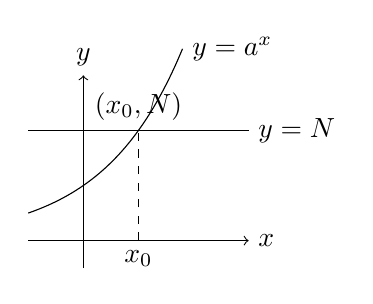
\begin{tikzpicture}[scale=0.7]
    % 绘制坐标轴
    \draw[->] (-1,0) -- (3,0) node[right] {$x$};
    \draw[->] (0,-0.5) -- (0,3) node[above] {$y$};
  
    % 绘制 y=2^x 曲线
    \draw[domain=-1:1.8,smooth,variable=\x] plot ({\x},{2^\x}) node[right] {$y=a^x$};
  
    % 绘制 y=2 直线
    \draw[smooth] (-1,2) -- (3,2) node[right] {$y=N$};
  
    % 标注交点和 (1,0)
    %\draw[dotted] (0,0) -- (1,0) node[below] {$1$};
    %\draw[dotted] (1,0) -- (1,{2^1}) node[midway,right] {$(1,2)$};
  
    % 连接交点和 (1,0) 的虚线
    \draw[dashed] (1,0) -- (1,{2^1});
  
    % 在 x 轴上方标注交点坐标
    \node[above] at (1,{2^1}) {$(x_0, N)$};
  
    % 在 x 轴下方标注 (1,0) 为 x_0
    \node[below] at (1,0) {$x_0$};
    \end{tikzpicture}
\end{minipage}

下面我们跟着定义来具体计算一些例子：
\begin{example}
    \ 

    $\log_24$

    $\log_2\frac{1}{2}$
\end{example}
在上面那个例子中我们注意到了形如
\begin{theorem}[对数恒等式]
    
\end{theorem}
\begin{example}
    $4^{\log_4 3}$
\end{example}
在实际使用中，有两种常用的对数——常用对数和自然对数。
\begin{definition}[自然对数与常用对数]
    

    \[\e:=\lim_{n\rightarrow +\infty}(1+\frac{1}{n})^n
    =\sum_{n=1}^{+\infty}\frac{1}{n!}\]
    \[\ln x \coloneqq \log _e x\]
    \[\lg x \coloneqq \log _{10} x\]
    $\lg(3x+2)$
\end{definition}

当然，以哪种对数为底并不是很重要
\begin{theorem}[换底公式]
    \[\log_a b=\frac{\log_c b}{\log_c a}\]
\end{theorem}
\begin{proof}
    
\end{proof}

\begin{theorem}[对数的运算法则]
    \ 

    $\forall M,N>0,a>0$且$a\ne1,n\in\mathbb{R}$，有
    \[\log_aN+\log_aM=\log_aMN\]
    \[\log_aM-\log_aN=\log_a\frac{M}{N}\]
    \[\log_aM^n=n\log_aM\]
\end{theorem}
\begin{proof}
    

    \qed
\end{proof}
\begin{example}[对数表的应用]
    
\end{example}
\begin{example}
    
\end{example}

\begin{corollary}
    
\end{corollary}
\clearpage
\subsection{对数函数}

\clearpage
\section{幂函数}
\subsection{幂函数的定义}
\clearpage
\subsection{指对幂函数的综合应用}
\clearpage
\chapter{三角函数}
\section{三角函数的基本认识}
\subsection{任意角与弧度制}
在讨论三角函数之前，我们应该更详细的定义什么是角。
毕竟当提起角，大家的脑子里第一反应还应该是锐角、直角、钝角、平角这样的分类。
一些人还会记得$360^\circ $的角叫做周角；
还有一些人会记得我们利用圆弧的平行概念，把在$(0^\circ,180^\circ)$内的角称为劣角，把在$(180^\circ,360^\circ)$内的角称为优角.
但是这些都没有顾及到大于$360^\circ$的角.因此我们要实用更加“动态”的角度去定义什么是角。
\begin{definition}[任意角]
    一条动射线绕其端点旋转到另一条定射线所得的图形叫做角，定射线和动射线分别叫做角的始边和终边。
    动射线的旋转方向有顺时针和逆时针之分，规定按顺时针方向旋转成的角是正角，按逆时针方向旋转而成的角叫做负角。
    当射线没有做任何旋转时，始边和终边重合，称之为零角。
\end{definition}

在这个定义中，我们进行了两点推广：一是加入了正负的概念，这有助于帮助我们解决角之间的运算；二是旋转的绝对量可以是任意的一个实数，这样我们就完成了任意角概念的推广。
\begin{example}\label{example7.1.1}
    \ 

$(1)$尝试画出$30^\circ$、$-140^\circ$、$460^\circ$、$-750^\circ$的角；

$(2)$解释$30^\circ+60^\circ$和$30^\circ-30^\circ$的几何意义.
\end{example}
\begin{jie}
    \ 

    $(1)$
    \begin{tikzpicture}
        \draw(1.5,0) coordinate (A) node[right] {A}
        -- (0,0) coordinate (B) node[left] {B}
        -- (30:1.5) coordinate (C) node[above right] {C}
        pic["$30^\circ$",draw=orange, ->, angle eccentricity=2, angle radius=0.5cm]
        {angle=A--B--C};
    \end{tikzpicture}
    \begin{tikzpicture}
        \draw(1.5,0) coordinate (A) node[right] {A}
        -- (0,0) coordinate (B) node[left] {B}
        -- (-140:1.5) coordinate (C) node[above right] {C}
        pic["$-140^\circ$",draw=orange, ->, angle eccentricity=1.5, angle radius=0.5cm]
        {angle=A--B--C};
    \end{tikzpicture}
    \begin{tikzpicture}
        \draw(1.5,0) coordinate (A) node[right] {A}
        -- (0,0) coordinate (B) node[left] {B}
        -- (460:1.5) coordinate (C) node[above right] {C}
        pic["$460^\circ$",draw=orange, ->, angle eccentricity=2, angle radius=0.5cm]
        {angle=A--B--C};
    \end{tikzpicture}
    \begin{tikzpicture}
        \draw(1.5,0) coordinate (A) node[right] {A}
        -- (0,0) coordinate (B) node[left] {B}
        -- (-750:1.5) coordinate (C) node[above right] {C}
        pic["$-750^\circ$",draw=orange, ->, angle eccentricity=2, angle radius=0.5cm]
        {angle=A--B--C};
    \end{tikzpicture}

    $(2)$
\end{jie}
\begin{zhu}
作出这样的约定：为不至于混淆，用希腊字母表示角时，我们会用$\alpha$,$\beta$代替$\angle \alpha,\angle \beta$，即省略掉$\angle$。
如果是用英文字母时，则分情况讨论.若某个点$A$仅是一个角的顶点，则这个角可以直接记作$A$;如果某个点$A$同时作为两个角$\angle CAB,\angle BAD$的顶点，则不应省略$\angle$。
\end{zhu}

可以看到，即使角的度数超过了$360^\circ$，画成图像也与我们过去的认知没有什么区别。这更多是给我们提供一种动态的视角去观察，也允许我们记录更多关于角度精确的信息。
一个简单的例子：体操运动员在空中转体三周半，即$1260^\circ$，这并不能等同于仅转了半周。同时，也为物理中圆周运动的研究提供了更多可能性。

但当回到平面上，只关心图像的时候，可以发现$30^\circ$，$390^\circ$，$-330^\circ$这三个角在图像上一模一样。在有相同起始边和顶点的时候，也具有相同的终边。
从旋转的角度看，从$30^\circ$到$390\du$，相当于顺时针旋转一周；从$30^\circ$到$-330^\circ$，相当于逆时针旋转一周.
它们都转了一圈回来了，相差一个$360^\circ$，这是旋转带来的一种天然的周期性。
我们也把这种公用一个终边，角度相差若干个$360$的一类角称为终边相同的角.注意，这里默认了始边和顶点是相同的，这会为我们的研究带来方便。
\begin{example}
    \ 

仍默认顶点和起始边相同，

    $(1)$写出终边与$30^\circ$角的终边相同的角构成的集合，把$30^\circ$换成$\alpha$呢？

    $(2)$判断下面三组角是否互为终边相同的角
\end{example}
\begin{jie}
    \ 
    
    $(1)$

    $(2)$


\end{jie}

为了方便研究，常常会把一个角放在平面直角坐标系中研究.一般地，我们会使角的顶点与坐标系原点重合，角的始边与坐标系横轴的非负半轴重合。
让终边在平面直角坐标系上转起来，就得到了各种各样的角.如果角的终边落在第$X$象限，则称这个角为第$X$象限角；当然，
如果角的终边落在了坐标轴上，它不再属于任一象限，就称之为坐标轴角了。下面我们看几个具体的例子。
\begin{example}
    \ 
    
    $(1)$指出例\ref{example7.1.1}$(1)$的四个角是位于何象限的角。

    $(2)$锐角一定是第一象限角吗？反之，第一象限角一定是锐角吗？
\end{example}
\begin{jie}
    \ 

    $(1)$

    $(2)$
\end{jie}

\begin{example}
    \ 

    \begin{enumerate}[(1)]
        \item a
        \item b
    \end{enumerate}

\end{example}


\clearpage
\subsection{任意角的三角函数}

\clearpage
\subsection{三角函数线及其应用*}
\clearpage
\subsection{同角三角函数关系}
在锐角三角函数中，
\begin{center}

\noindent
\begin{minipage}[t]{0.7\textwidth}
    \vspace{0pt} % 垂直对齐到顶部
    \begin{tikzpicture}[scale=2]
        % Define coordinates
        \coordinate (A) at (0,0);
        \coordinate (B) at (1.732,0);
        \coordinate (C) at (0,1);
        
        % Draw triangle
        \draw (A) -- (B) -- (C) -- cycle;
        
        % Label vertices
        \node[left] at (A) {$A$};
        \node[right] at (B) {$B$};
        \node[above] at (C) {$C$};
        
        % Draw right angle symbol
        \draw ($(A)!4pt!(C)$) -- ++(4pt,0) -- ++(0,-4pt);
    \end{tikzpicture}
\end{minipage}%
\begin{minipage}[t]{0.25\textwidth}
    \vspace{-\baselineskip} % 移除一个基线
    \begin{align*}
    &\sin B =\frac{AC}{BC}\\
    &\cos B =\frac{AB}{BC}\\
    &\tan B =\frac{AC}{AB}\\
    &AB^2+AC^2=BC^2
    \end{align*}
   
\end{minipage}
    
\end{center}


\clearpage
\subsection{诱导公式}\label{subsec_诱导公式}
\clearpage
\section{三角函数的图像}
\subsection{正弦函数、余弦函数的图像与性质}
\clearpage
\subsection{\texorpdfstring{$A\sin(\omega x+\varphi)+h$}s的图像与性质}%\texorpdfstring命令后面要加一个被吞掉的字符
在上一节中详细地介绍了\(\sin x \)与\(\cos x\)的图像，接下来就可以将过去学习的伸缩变换、平移变换作用到三角函数上，看看会有什么新的变化。
\begin{example}
    在同一直角坐标系中绘制\(y=\sin ,y=2\sin x\)的图像。
\end{example}
\begin{example}
    在同一直角坐标系中绘制\(y=\sin x,y=\sin 2x\)的图像。
\end{example}
\begin{example}
    在同一直角坐标系中绘制\(y=\sin x,y=\sin (x+\dfrac{\pi}{3})\)的图像。
\end{example}
\begin{example}
    在同一直角坐标系中绘制\(y=\sin x,y=\sin x+1\)的图像。
\end{example}
\begin{example}
    在同一直角坐标系中绘制\(y=\sin x,y=\sin(2x+\dfrac{\pi}{3})\)的图像。
\end{example}

\begin{example}
    \(f(x)=\sin(\omega x +\dfrac{\pi}{4})\)\((\omega>0)\)在\((\dfrac{\pi}{2},\dfrac{3\pi}{2})\)内没有最值，
    求\(\omega\)的取值范围。
\end{example}


\begin{example}[2022年全国甲卷]
    设函数 \( f(x) = \sin(\omega x + \dfrac{\pi}{3}) \) 在区间 \( (0, \pi) \) 恰有三个极值点、两个零点，求 \(\omega\) 的取值范围
\end{example}

\begin{example}[2016年新课标I卷]
    已知函数 \( f(x) = \sin(\omega x + \varphi) \left(\omega > 0, \ |\varphi| \leq \dfrac{\pi}{2}\right) \)，
    \( x = -\dfrac{\pi}{4} \) 为 \( f(x) \) 的零点，\( x = \dfrac{\pi}{4} \) 为 
    \( y = f(x) \) 图象的对称轴，且 \( f(x) \) 在 \( (\dfrac{\pi}{18}, \dfrac{5\pi}{36}) \) 上单调，求\(\omega\) 的最大值。
\end{example}


\begin{example}
已知函数 \( f(x) = 2\sin(\omega x + \varphi) \) (\(\omega > 0\)) 的图象关于直线 \( x = \dfrac{\pi}{3} \) 对称, 且 \( f\left(\dfrac{\pi}{12}\right) = 0 \), 求 \(\omega\) 的最小值为

\end{example}
\begin{exercise}
已知函数 \( f(x) = A\sin(\omega x + \varphi) \) (\(A > 0, \omega > 0, |\varphi| \leq \dfrac{\pi}{2}\))，满足 \( f\left(-\dfrac{\pi}{6}\right) = 0 \) 且 \(\forall x \in \mathbb{R} \) 都有 \( f(x) = f\left(\dfrac{2\pi}{3} - x\right) \)，若 \( f(x) \) 在 \( \left(\dfrac{5\pi}{36}, \dfrac{2\pi}{9}\right) \) 上单调，求\(\omega\) 的最大值为
\end{exercise}






















\clearpage
\subsection{正切函数的图像与性质}
\clearpage
\subsection{\texorpdfstring{$A\tan(\omega x+\varphi)+h$}s的图像与性质}
\clearpage
\subsection{余切、正割、余割函数的图像与性质**}
\clearpage
\subsection{反三角函数的图像与性质**}
\clearpage
\review





\clearpage
\hw
\begin{homework}[2012年新课标卷]
    已知 \(\omega > 0\)，函数 \( f(x) = \sin(\omega x + \dfrac{\pi}{4}) \) 在区间 \((\dfrac{\pi}{2}, \pi)\) 上单调递减，则实数 \(\omega\) 的取值范围是（\quad  ）

\begin{table}[H]
    \centering
\begin{tabular*}{\hsize}{@{}@{\extracolsep{\fill}}llll@{}}
   \(\text{A.}  \left[\dfrac{1}{2}, \dfrac{5}{4}\right] \)  & \( \text{B.}  \left[\dfrac{1}{2}, \dfrac{3}{4}\right] \) & \(    \text{C.} \left(0, \dfrac{1}{2}\right] \) & $\text{D.}  (0, 2]$
\end{tabular*}
\end{table}

\end{homework}

\begin{homework}
函数 \( f(x) = \sin\left(\omega x + \dfrac{\pi}{3}\right) \)   $ (\omega > 0)$ 在 \( \left(0, \dfrac{\pi}{3}\right) \) 单调递增，\(\omega\) 的取值范围为\_\_\_\_\_。
\end{homework}

\begin{homework}[2016天津卷]
    已知函数 \( f(x) = \sin\left(\omega x - \dfrac{\pi}{4}\right) (\omega > 0) \)，若 \( f(x) \) 在区间 \( (\pi, 2\pi) \) 内没有零点，则 \(\omega\) 的取值范围是（\quad ）

\begin{table}[H]
    \centering
\begin{tabular*}{\hsize}{@{}@{\extracolsep{\fill}}llll@{}}
  $\text{A.}  \left(0, \dfrac{1}{8}\right] $ & $\text{B.}\left(0, \dfrac{1}{4}\right] \cup \left[\dfrac{5}{8}, 1\right) $ & $\text{C.} \left(0, \dfrac{5}{8}\right] $&$\text{D.} (0, 8] \cup \left[\dfrac{1}{4}, \dfrac{5}{8}\right]$
\end{tabular*}
\end{table}

\end{homework}
\begin{homework}
  函数 \( f(x) = \sin\left(\omega x - \frac{\pi}{6}\right) \) $( \omega > 0)$ 在 \( (0, 2\pi) \) 有且仅有一个零点，则 \(\omega\) 的取值范围为\_\_\_\_\_。
\end{homework}
\begin{homework}
函数 \( f(x) = \cos\left(\omega x + \frac{\pi}{6}\right) \)   $( \omega > 0)$ 在 \( \left(-\frac{\pi}{3}, \frac{\pi}{2}\right) \) 有且仅有$ 1$ 个零点，\(\omega\) 的取值范围为\_\_\_\_\_。
\end{homework}
\begin{homework}
    函数 \( f(x) = \sin\left(\omega x + \frac{\pi}{6}\right) \) 在 \( \left(-\frac{\pi}{2}, 0\right) \) 没有零点，\(\omega\) 的取值范围为\_\_\_\_\_。
\end{homework}
\begin{homework}[2018北京卷理]
 设函数 \( f(x) = \cos\left(\omega x - \dfrac{\pi}{6}\right) \) (\(\omega > 0\))。若 \( f(x) \leq f\left(\frac{\pi}{4}\right) \) 对任意的实数 \( x \) 都成立，则 \(\omega\) 的最小值为\_\_\_\_\_。
\end{homework}
\begin{homework}
    已知函数 \( f(x) = 6\cos(\omega x + \varphi) (\omega > 0, 0 < \varphi < \pi) \)，\( \forall x \in \mathbb{R} \) 都有 \( f(x) \leq |f\left(\dfrac{\pi}{6}\right)| \)，且 \( x = -\dfrac{\pi}{6} \) 是 \( f(x) \) 的一个零点。若 \( g(x) = f(x) - 6 \) 在 \( \left(\dfrac{\pi}{15}, \dfrac{\pi}{6}\right) \) 上有且只有一个零点，则 \(\omega\) 的最大值为\_\_\_\_\_。
\end{homework}
\begin{homework}
    
\end{homework}
\begin{homework}
    
\end{homework}
\begin{homework}
    
\end{homework}
\begin{homework}
    
\end{homework}
\begin{homework}
    
\end{homework}
\begin{homework}
    
\end{homework}
\begin{homework}
    
\end{homework}
\begin{homework}
    
\end{homework}
\begin{homework}
    
\end{homework}
\begin{homework}
    
\end{homework}




\clearpage

\section{三角恒等变换}
\subsection{两角和、差的三角函数}
    \ref{subsec_诱导公式}节诱导公式说明了$\alpha$与$\pm \alpha \pm \frac{n\pi}{2}$的三角函数关系。
    ，但如果\(\frac{\pi}{2}\)变为一个特殊的角呢？对于一般的情况，是否有
    \[\cos(\alpha+\beta) = \cos \alpha+cos \beta\]
    这样美好的公式呢？带入几个特殊的角，发现这是不可能的……下面这个定理给出真正的两角和的余弦公式。
\begin{theorem}[两角和的余弦]\label{两角和余弦定理}
    $\forall \alpha,\beta \in \mathbb{R} $满足
    \begin{equation}
        \cos(\alpha+\beta) = \cos \alpha\cos \beta -\sin \alpha\cos \beta  
    \end{equation}
\end{theorem}
\begin{proof}
    先考虑$\alpha,\beta$都是锐角的情况。在单位圆中画出$\aa$，$\bb$和$-\bb$。
    \begin{figure}[htbp]
    \centering
    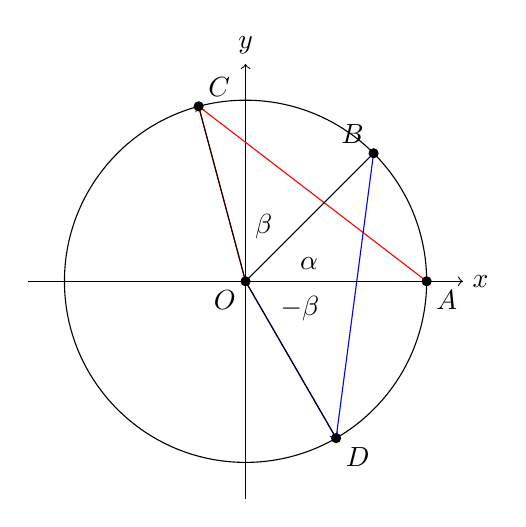
\begin{tikzpicture}[scale=2.3]
      \coordinate (O) at (0,0);
      \draw[->] (-1.2,0) -- (1.2,0) node[right] {$x$};
      \draw[->] (0,-1.2) -- (0,1.2) node[above] {$y$};
      \draw (0,0) circle [radius=1];
      \coordinate (A) at (1,0);
      \coordinate (B) at (0.707,0.707);
      \coordinate (C) at (-0.259,0.966);
      \coordinate (D) at (0.5,-0.866);
      \draw[->,red] (O) -- (C);
      \draw[->,blue] (O) -- (D);
      \draw[red] (A) -- (C);
      \draw[blue] (B) -- (D);
      \draw (O) -- (A) node[midway,below] {};
      \draw (O) -- (B) node[midway,left] {};
      \draw (O) -- (C) node[midway,above left] {};
      \draw (O) -- (D) node[midway,below left] {};
      \fill (O) circle (0.8pt) node[below left] {$O$};
      \fill (A) circle (0.8pt) node[below right] {$A$};
      \fill (B) circle (0.8pt) node[above left] {$B$};
      \fill (C) circle (0.8pt) node[above right] {$C$};
      \fill (D) circle (0.8pt) node[below right] {$D$};
      \node at (0.35,0.1) {$\alpha$};
      \node at (0.1,0.3) {$\beta$};
      \node at (0.3,-0.15) {$-\beta$};
    \end{tikzpicture}
    \end{figure}

    其中$A(1,0)$，$B(\cos\aa,\sin\aa)$，$C(\cos(\aa+\bb),\sin(\aa+\bb))$，$D(\cos(-\bb),\sin(-\bb))=(\cos\bb,-\sin\bb)$。
    由于圆的半径相等，$\angle AOC=\angle BOD=\aa+\bb$，故$\triangle AOC\cong \triangle BOD(SAS)$，
    因此有$|AC|=|BD|$。
    
    即
    \begin{align*}
        (\cos^2(\aa+\bb)-1)^2+\sin^2(\aa+\bb)&=(\cos\aa-\cos\bb)^2+(\sin\aa+\sin\bb)^2\\
        \cos^2(\aa+\bb)-2\cos(\aa+\bb)+1+\sin^2(\aa+\bb)&=\cos^2\aa-2\cos\aa\cos\bb+\cos^2\bb+\sin^2\aa+2\sin\aa\sin\bb+\sin^2\bb\\
        1-2\cos(\aa+\bb)+1&=1+1-2\cos\aa\cos\bb+2\sin\aa\sin\bb\\
        \cos(\alpha+\beta)& = \cos \alpha\cos \beta -\sin \alpha\cos \beta  
    \end{align*}

    在这里用到了之前证明过的$\sin^2\aa+\cos^2\bb=1\quad(\forall\aa\in\mathbb{R})$.
\end{proof}

接下来就可以利用定理\ref{两角和余弦定理}来证明接下来的五个式子
\begin{theorem}
    $\forall \alpha,\beta \in \mathbb{R} $满足
    \begin{equation}\label{两角差余弦}
        \cos(\alpha-\beta) = \cos \alpha\cos \beta +\sin \alpha\cos \beta  
    \end{equation}
    \begin{equation}\label{两角和正弦}
        \sin(\aa+\bb)=\sin\aa\cos\bb+\cos\aa\sin\bb
    \end{equation}
    \begin{equation}\label{两角差正弦}
        \sin(\aa-\bb)=\sin\aa\cos\bb-\cos\aa\sin\bb
    \end{equation}
    \begin{equation}\label{两角和正切}
        \tan(\aa+\bb)=\frac{\tan\aa+\tan\bb}{1-\tan\aa\tan\bb}
    \end{equation}
    \begin{equation}\label{两角差正切}
        \tan(\aa-\bb)=\frac{\tan\aa-\tan\bb}{1+\tan\aa\tan\bb}
    \end{equation}
\end{theorem}
\begin{proof}
仅证明
\end{proof}

\clearpage
\subsection{二倍角公式及其拓展}
\clearpage
\subsection{积化和差与和差化积}
\begin{theorem}
    \begin{equation}
        \sin\alpha \sin\beta = \frac{1}{2}[\cos(\alpha - \beta) - \cos(\alpha + \beta)]
    \end{equation}
        
    \begin{equation}
        \cos\alpha \cos\beta = \frac{1}{2}[\cos(\alpha - \beta) + \cos(\alpha + \beta)]
    \end{equation}
        
    \begin{equation}
        \sin\alpha \cos\beta = \frac{1}{2}[\sin(\alpha + \beta) + \sin(\alpha - \beta)]
    \end{equation}
        
    \begin{equation}
        \cos\alpha \sin\beta =\frac{1}{2} [\sin(\alpha + \beta) - \sin(\alpha - \beta)]
    \end{equation}
\end{theorem}
\begin{theorem}
    

    \begin{equation}
        \sin\alpha + \sin\beta = 2 \sin\left(\frac{\alpha + \beta}{2}\right) \cos\left(\frac{\alpha - \beta}{2}\right)
    \end{equation}
        
    \begin{equation}
        \sin\alpha - \sin\beta = 2 \cos\left(\frac{\alpha + \beta}{2}\right) \sin\left(\frac{\alpha - \beta}{2}\right)
    \end{equation}
        
    \begin{equation}
        \cos\alpha + \cos\beta = 2 \cos\left(\frac{\alpha + \beta}{2}\right) \cos\left(\frac{\alpha - \beta}{2}\right)
    \end{equation}
        
    \begin{equation}
        \cos\alpha - \cos\beta = -2 \sin\left(\frac{\alpha + \beta}{2}\right) \sin\left(\frac{\alpha - \beta}{2}\right)
    \end{equation}
\end{theorem}

\begin{example}
    求满足下列条件的区域的面积：
    \[\{(x,y)|x,y\in[0,\frac{\pi }{2}],\sin ^2 x-\sin x \sin y+\sin ^2y\leq\frac{3}{4}\}\]
\end{example}

\begin{jie}
\begin{way1}
    对不等式左侧的式子做变换
\begin{align}
     &\sin ^2 x-\sin x \sin y+\sin ^2y \notag\\ 
     =&\frac{1}{2}(1-\cos 2x-(\cos(x-y)-\cos(x+y))+1-\cos2y)\label{积化和差求面积1}\\
     =&\frac{1}{2}(2-2\cos(x+y)\cos(x-y)-\cos(x-y)+\cos(x+y))\label{积化和差求面积2}
\end{align}
   式\ref{积化和差求面积1}是对\(\sin x\sin y\)作积化和差得到的的
   ，式\ref{积化和差求面积2}是对\(\cos 2x+\cos 2y\)作和差化积得到的。
   
   故原不等式可以变为
   \[2\cos(x+y)\cos(x-y)+\cos(x-y)-\cos(x+y)-\frac{1}{2}\geq 0\]
   因式分解得
   \[(2\cos(x+y)+1)(\cos(x-y)-\frac{1}{2})\geq 0\]
   解得
 \begin{equation}\label{积化和差求面积3}
      \left\{\begin{array} { l } 
       \displaystyle{ \cos(x + y) \leqslant -\frac { 1 } { 2 }  } \\
       \displaystyle{ \cos(x - y) \leqslant \frac{1}{2}}
       \end{array} \text { 或 } \left\{\begin{array}{l}
       \displaystyle\cos(x + y) \geqslant -\frac { 1 } { 2 } \\
       \displaystyle\cos(x - y) \geqslant \frac{1}{2}
       \end{array}\right.\right.
 \end{equation}

    由于\(x,y\in[0,\dfrac{\pi }{2}]\)，故可以确定
    \[0\leq x+y\leq\pi,-\frac{\pi}{2}\leq x-y\leq \frac{\pi}{2}\]

    结合不等式组\ref{积化和差求面积3}，列出下面的不等式组
   \[\left\{\begin{array} { l } 
    \displaystyle{0 \leq x + y \leqslant \frac { 2 } { 3 }\pi  } \\
    \displaystyle{-\frac{\pi}{3} \leq x - y \leq \frac { \pi } { 3 } }
    \end{array} \text { 或 } \left\{\begin{array}{l}
    \displaystyle \frac{2 }{3}\pi\leq x+y \leq \pi \\
    \displaystyle\frac{\pi}{3}\leq x-y  \leq \frac{\pi}{2} \text{或}-\frac{\pi}{2}\leq x-y  \leq -\frac{\pi}{3}
    \end{array}\right.\right.\]

    如下图所示在平面直角坐标系中绘制出两个不等式组对应的区域：
    %\sout{思考：请利用此题计算}\[{\sum_{n=1}^{+\infty}\frac{1}{n^2}}\]

    \begin{figure}[h]
        \centering
        
        \begin{subfigure}[h]{0.45\textwidth}
            \centering
            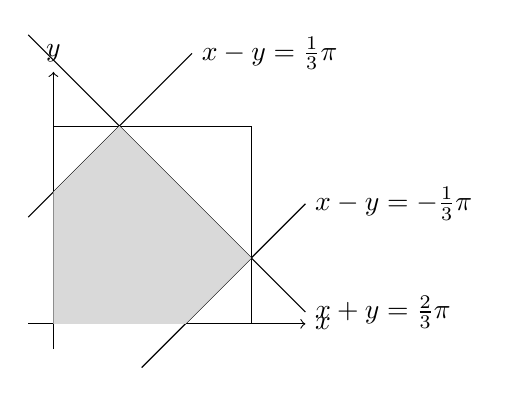
\begin{tikzpicture}[
                scale=1.6, % 调整比例
            ]
            % 定义坐标轴
            \draw[->] (-0.2,0) -- (2,0) node[right] {$x$};
            \draw[->] (0,-0.2) -- (0,2) node[above] {$y$};
            \draw (0,0) rectangle (1.57,1.57);
            % 定义直线的坐标
            \def\lineA{(-0.2, {2/3*3.14159 +0.2}) -- (2, {2/3*3.14159 -2})}
            \def\lineB{(-0.2, {1/3*3.14159 -0.2}) -- (1.1, {1/3*3.14159 + 1.1})}
            \def\lineC{(0.7, {-1/3*3.14159+0.7}) -- (2, {-1/3*3.14159 + 2})}
            
            % 画直线
            \draw \lineA node[right] {$x+y=\frac{2}{3}\pi$};
            \draw \lineB node[right] {$x-y=\frac{1}{3}\pi$};
            \draw \lineC node[right] {$x-y=-\frac{1}{3}\pi$};
            
            % 填充灰色区域
            \coordinate (A) at (0,0);
            \coordinate (B) at (0,{pi/3});
            \coordinate (C) at ({pi/6},{pi/2});
            \coordinate (D) at ({pi/2},{pi/6});
            \coordinate (E) at ({pi/3},0); % 闭合路径
            \fill[gray!30] (A) -- (B) -- (C) -- (D) -- (E)--cycle;
            \end{tikzpicture}
            \caption{情况1}
        \end{subfigure}%
        \hfill
        \begin{subfigure}[h]{0.45\textwidth}
            \centering
            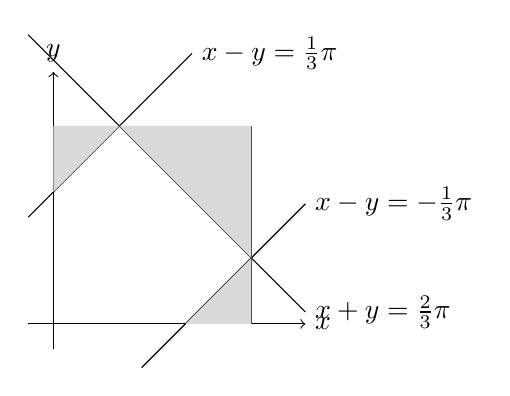
\begin{tikzpicture}[
                scale=1.6, % 调整比例
            ]
            % 定义坐标轴
            \draw[->] (-0.2,0) -- (2,0) node[right] {$x$};
            \draw[->] (0,-0.2) -- (0,2) node[above] {$y$};
            \draw (0,0) rectangle (1.57,1.57);
            % 定义直线的坐标
            \def\lineA{(-0.2, {2/3*3.14159 +0.2}) -- (2, {2/3*3.14159 -2})}
            \def\lineB{(-0.2, {1/3*3.14159 -0.2}) -- (1.1, {1/3*3.14159 + 1.1})}
            \def\lineC{(0.7, {-1/3*3.14159+0.7}) -- (2, {-1/3*3.14159 + 2})}
            
            % 画直线
            \draw \lineA node[right] {$x+y=\frac{2}{3}\pi$};
            \draw \lineB node[right] {$x-y=\frac{1}{3}\pi$};
            \draw \lineC node[right] {$x-y=-\frac{1}{3}\pi$};
            
            % 填充灰色区域
            \coordinate (A) at (0,0);
            \coordinate (B) at (0,{pi/3});
            \coordinate (C) at ({pi/6},{pi/2});
            \coordinate (D) at ({pi/2},{pi/6});
            \coordinate (E) at ({pi/3},0);
            \coordinate (F) at (0,{pi/2}); % 闭合路径
            \coordinate (G) at ({pi/2},{pi/2});
            \coordinate (H) at ({pi/2},0);
            \fill[gray!30] (B) -- (F) -- (C)--cycle;
            \fill[gray!30] (C) -- (G) -- (D)--cycle;
            \fill[gray!30] (D) -- (H) -- (E)--cycle;
            \end{tikzpicture}
            \caption{情况2}
        \end{subfigure}
        \caption{由上不等式组绘制出的图像}
        \label{积化和差求面积图像}
    \end{figure}

    上图中情况1对应着左侧的不等式组，灰色阴影部分为各个不等式的交集，即为题目所求区域
    ；情况2对应着右侧的不等式组，最后要求取三个灰色部分的交集，这是不可能的，故无解。

 综上所述，最终原题目中的面积为正方形面积减去三个三角形面积：
    \[S=\left(\frac{\pi}{2}\right)^2-2\times\frac{1}{2}\left(\frac{\pi}{6}\right)^2-\frac{1}{2}\left(\frac{\pi}{3}\right)^2=\frac{\pi^2}{6}\]
\end{way1}

\begin{way2}
    仅仅考虑边缘部分，
    \begin{equation}
        \sin^2 x-\sin x\sin y+\sin^2 y=\frac{3}{4}
    \end{equation}
    对其配方\footnote{这个操作不太习惯也没关系，在二次型可以学习到类似的技巧。}，得到
    \begin{equation}
        \frac{1}{3}(\sin x +\sin y)^2+(\sin y-\sin x)^2=1
    \end{equation}
    不妨设
    \[
   \left\{
        \begin{array} { l } 
        \sin x+\sin y=\sqrt{3} \sin t\\
        \sin y-\sin x=\cos t
        \end{array}
    \right.
    \]
    解得
        \[
   \left\{
        \begin{array} { l } 
        \displaystyle \sin x=\frac{1}{2}(\sqrt{3} \sin t-\cos t)=\sin(t-\frac{\pi}{6})\\
        \displaystyle \sin y=\frac{1}{2}(\sqrt{3} \sin t+\cos t)=\sin(t+\frac{\pi}{6})
        \end{array}
    \right.
    \]

    利用正弦函数的性质脱掉\(\sin\)的外壳得到：
    \begin{equation}\label{积化和差求面积方程1}
        x=t-\frac{\pi}{6}+2k\pi\ (k\in \mathbb{Z})
    \end{equation}
    \begin{equation}\label{积化和差求面积方程2}
        x+t-\frac{\pi}{6}=\pi+2k\pi\ (k\in \mathbb{Z})
    \end{equation}
    \begin{equation}\label{积化和差求面积方程3}
        y=t+\frac{\pi}{6}+2k\pi\ (k\in \mathbb{Z})
    \end{equation}
    \begin{equation}\label{积化和差求面积方程4}
        y+t+\frac{\pi}{6}=\pi+2k\pi\ (k\in \mathbb{Z})
    \end{equation}
    两两消去参数\(t\)得到三组平行直线系方程：
    \begin{equation}
        y-x=\frac{\pi}{3}+2k\pi  \ (\ref{积化和差求面积方程3}-\ref{积化和差求面积方程1},k\in \mathbb{Z})
    \end{equation}
    \begin{equation}
        x+y=\frac{2}{3}\pi+2k\pi \ (\ref{积化和差求面积方程1}+\ref{积化和差求面积方程4}\text{或}\ref{积化和差求面积方程2}+\ref{积化和差求面积方程3},k\in \mathbb{Z})
    \end{equation}
    \begin{equation}
        x-y=\frac{\pi}{3}+2k\pi\ (\ref{积化和差求面积方程2}-\ref{积化和差求面积方程4},k\in \mathbb{Z})
    \end{equation}


    结合\(x,y\in[0,\dfrac{\pi}{2}]\)，即可确定是
    \[x-y+\frac{\pi}{3}=0\]
    \[x-y-\frac{\pi}{3}=0\]
    \[x+y-\frac{2}{3}\pi=0\]仍然可以绘制出图\ref{积化和差求面积图像}，但是这仅仅确定了边界，具体是哪块区域
    可以通过代入特殊点来确定。
\end{way2}

\begin{way3}
同法2一样，仍然先考虑边界。注意到原式的形式类似余弦定理
\end{way3}



\end{jie}




\clearpage
\subsection{三角函数的其他定义*}
\clearpage
\subsection{反三角函数的恒等变换**}
\clearpage
\review
\clearpage
\hw
\clearpage
\chapter{函数的应用}
\section{函数的应用（一）}
\subsection{函数的零点}
\clearpage
\subsection{Cauchy方程简介*}
%\subsubsection{从\texorpdfstring{$f(x+y)=f(x)+f(y)$}s开始}
\begin{theorem}
    若\(y=f(x), x\in \mathbb{R}\)连续，且满足Cauchy加性方程
    \begin{equation}
        f(x+y)=f(x)+f(y)
    \end{equation}
    则函数必然为正比例函数\[f(x)=cx\]
    其中\(c=f(1)\)。
\end{theorem}
\clearpage
\section{函数的应用（二）}
\subsection{函数的增长速度}
\clearpage
\subsection{函数模型}
\clearpage
\section{解三角形}
解三角形，就是给定若干三角形的元素，确定出三角形其他元素的过程。一个自然的问题是，究竟
什么样的条件才能唯一确定一个三角形，或者退一步，允许一两个多解的存在？
在初中阶段就学习了全等三角形的判定条件：$SSS,SAS,ASA,AAS,HL$。也就是说
当给出这些条件时，应当能唯一一个三角形。而$SSA$这样的条件，虽然不能确定唯一一个三角形，
但是解也不会超过两个。但这些仅是定性地判断存在性，如何具体计算它们的数值呢？

例如，理论上给出两边及其夹角，其余的一角两边应当随之确定。可是要如何计算呢？
这些问题就由正弦定理和余弦定理来解决。

\subsection{正弦定理}
\begin{example}
    给定一个$\rt \triangle ABC$，\(\angle C =\dfrac{\pi}{2}\)，\(\angle A=\dfrac{\pi}{6}\)，
    \(AB=2\)。请尝试确定三角形其余一角和两边，以及外接圆的半径。
\end{example}
\begin{jie}
    
\end{jie}
\begin{theorem}[正弦定理]
  \begin{equation}
      \frac{a}{\sin A}=\frac{b}{\sin B }=\frac{c}{\sin C}=2R
  \end{equation}
\end{theorem}
\clearpage
\subsection{余弦定理}
\begin{theorem}[余弦定理]
\begin{equation}
    a^2=b^2+c^2-2bc\cos A
\end{equation}
\begin{equation}
    b^2=a^2+c^2-2ac\cos B
\end{equation}
\begin{equation}
    c^2=a^2+b^2-2ab\cos C
\end{equation}
\end{theorem}
\clearpage
\subsection{正余弦定理的综合应用}
\begin{example}
    在\(\tri ABC\)中，\(AB=1\)，\(AC=2\)，\(\angle BAC=\theta\)。再取一点\(D\)，使得
    \(\tri BCD\)为等边三角形。求线段\(AD\)长的最大值。
\end{example}
\begin{analyse}
    要求\(AD\)的长度，总是避不开\(\angle ACB\)或者\(\angle ABC\)，无法直接用\(\theta\)。但是
    当两边及其夹角确定的时候，整个三角形应该是唯一确定的，故可以用已有的两边及其夹角表示出其他量。
\end{analyse}
\begin{jie}
    通过绘图可知\(\theta\in(0,\pi)\)，最后\(AD\)的长度应当是\(\theta\)的函数。
    不妨设\(\angle BCA=\varphi\)

    在\(\tri ABC\)中，由正弦定理得\[\frac{BC}{\sin\theta}=\frac{AB}{\sin\varphi}\]
    即\[\sin\varphi=\frac{\sin\theta}{BC}\]

    在\(\tri ABC\)中，由射影定理得\[AC=AB\cos\theta+BC\cos\varphi\]
    即\[\cos\varphi=\frac{2-\cos\theta}{BC}\]

    在\(\tri ABC\)中，由余弦定理得
    \begin{align*}
         BC^2&=AC^2+AB^2-2AB\cdot AC\cos\theta\\
            &=5-4\cos\theta
    \end{align*}
   
    在\(\tri ACD\)中，$CD=BC$，再由余弦定理得
    \begin{align*}
        AD^2&=AC^2+CD^2-2AC\cdot CD\cos(\varphi+\frac{\pi}{3})\\
            &=4+BC^2-4BC(\cos\varphi\cos\frac{\pi}{3}-\sin\varphi\sin\frac{\pi}{3})\\
            &=4+5-4\cos\theta-4(\frac{2-\cos\theta}{2}-\frac{\sqrt{3}\sin\theta}{2})\\
            &=5+2\sqrt{3}\sin\theta-2\cos\theta\\
            &=5+\sqrt{(2\sqrt{3})^2+2^2}(\frac{\sqrt{3}}{2}\sin\theta-\frac{1}{2}\cos\theta)\\
            &=5+4\sin(\theta-\frac{\pi}{6})\\
            &\leq9
    \end{align*}
    等号当\(\theta=\dfrac{2}{3}\pi\)时取得

\end{jie}


\begin{example}
    在 $ \triangle A B C$  中，角 $ A, B, C$  所对的边分别为$  a, b, c $ ，
    且外接圆半径为 $ R=5 $ ，求$ \dfrac{a b c}{a^{2}+b^{2}+2 c^{2}} $ 的最大值为   
\end{example}

\begin{jie}
    \[
\begin{aligned}
    \frac{abc}{a^2 + b^2 + 2c^2} &= \frac{ab \cdot 2 \times 5 \sin C}{a^2 + b^2 + 2(a^2 + b^2 - 2ab \cos C)}\\
                                & = \frac{10ab \sin C}{3(a^2 + b^2) - 4ab \cos C}\\
                               &  \leq \frac{10ab \sin C}{6ab - 4ab \cos C} = \frac{5 \sin C}{3 - 2 \cos C} \\
                               &\leq \frac{5 \sin C}{\sqrt{5} \sin C} = \sqrt{5}.
\end{aligned}
\]
\qed
\end{jie}
\begin{theorem}[Weisenböck不等式]
    在\(\tri ABC\) 中，角 $ A, B, C$  所对的边分别为$  a, b, c $ ，三角形面积为\(S\)对任意实数 $ x, y, z $ ，满足 $ x+y+z>0,  x y+y z+z x>0$  ，则有

$$x a^{2}+y b^{2}+z c^{2} \geqslant 4 \sqrt{x y+y z+z x} S$$


当且仅当 $ \cot A: \cot B: \cot C=x: y: z$  时取得等号．
\end{theorem}
\begin{proof}
    \[\begin{aligned}
        x a^{2}+y b^{2}+z c^{2} & =x a^{2}+y b^{2}+z\left(a^{2}+b^{2}-2 a b \cos C\right) \\
        & =(x+z) a^{2}+(y+z) b^{2}-2 z a b \cos C \\
        & \geqslant 2 \sqrt{(x+z)(y+z)} a b-2 z a b \cos C \\
        & =2 a b(\sqrt{(x+z)(y+z)}-z \cos C) \\
        & \geqslant 2 a b\left(\sqrt{(x+z)(y+z)-z^{2}} \sin C\right) \\
        & =4 S_{\triangle} \sqrt{x y+y z+z x}
        \end{aligned}\]

        当且仅当 $ \frac{a^{2}}{x+y}=\frac{b^{2}}{y+z}=\frac{c^{2}}{z+x} $ 亦即 $ x: y: z=\cot A: \cot B: \cot C $ 时取得等号．
    \[m \sin \theta+n \cos \theta \leqslant \sqrt{m^{2}+n^{2}} \Longleftrightarrow \sqrt{m^{2}+n^{2}}-n \cos \theta \geqslant m \sin \theta\]
        \qed
\end{proof}
\clearpage